  \chapter{LaTeX Examples}

This template is based on the Standard \LaTeX{} book class, so the options of book class work as well (Note that the option of papersize has no effect due to \lstinline{device} option). The default encoding is UTF-8 while \TeX{} Live is recommended. The test environment is Win10 + \TeX{} Live 2019, either \lstinline{PDFLaTeX} or \lstinline{XeLaTeX} works fine.

\section{Definitions, Theorems, and Propositions}
section{Theorem Class Environments}

In this template, we defined four different theorem class environments

\begin{itemize}
\item \textit{Theorem Environment}, including title and content, numbering corresponding to chapter. Three types depending on the format:
   \begin{itemize}
      \item \textcolor{main}{\textbf{definition}} environment, the color is  \textcolor{main}{main};
      \item \textcolor{second}{\textbf{theorem, lemma, corollary}} environment, the color is \textcolor{second} {second};
      \item \textcolor{third}{\textbf{proposition}} environment, the color is \textcolor{third}{third}.
   \end{itemize}
\item \textit{Example Environments}, including \textbf{example, exercise, problem} environment, auto numbering corresponding to chapter.
\item \textit{Proof Environment}, including \textbf{proof, note} environment containing introductory symbol (\textbf{note} environment) or ending symbol (\textbf{proof} environment).
\item \textit{Conclusion Environments}, including \textbf{conclusion, assumption, property, remark, solution}\footnote{We also define an option \lstinline{result}, which can hide the \lstinline{solution} and \lstinline{proof} environments. You can switch between \lstinline{result=answer} and \lstinline{result=noanswer}} environment, all of which begin with boldfaced words, with format consistent with normal paragraphs.
\end{itemize}

\subsection{Theorem Class Environments}
Since the template uses the \lstinline{tcolorbox} package to customize the theorem class environments, it is slightly different from the normal theorem environments. The usage is as follows:
\begin{lstlisting}
\begin{theorem}{<theorem name>}{<label>}
The content of theorem.
\end{theorem}
\end{lstlisting}

The first parameter \lstinline{<theorem name>} represents the name of the theorem, and the second parameter \lstinline{label} represents the label used in cross-reference with \verb|ref{thm:label}|. Note that cross-references must be prefixed with \lstinline{thm:}. 

Other theorem class environments with the same usage includes:

\begin{table}[htbp]
   \centering
   \caption{Theorem Class Environments}
     \begin{tabular}{llll}
     \toprule
     Environment & Label text & Prefix & Cross-reference \\
     \midrule
     definition & label & def   & \lstinline|\ref{def:label}| \\
     theorem & label & thm   & \lstinline|\ref{thm:label}| \\
     lemma & label & lem   & \lstinline|\ref{lem:label}| \\
     corrlary & label & cor   & \lstinline|\ref{cor:label}| \\
     proposition & label & pro   & \lstinline|\ref{pro:label}| \\
     \bottomrule
     \end{tabular}%
   \label{tab:theorem-class}%
 \end{table}%
 
\subsection{Other Customized Environments}

The other three math environments can be called directly since there are no additional option for them, e.g. \lstinline{example}:
\begin{lstlisting}
\begin{example}
This is the content of example environment.
\end{example}
\end{lstlisting}

The effect is as follows:

\begin{example}
This is the content of example environment.
\end{example}

These are all similar environments with slight differences lies in:

\begin{itemize}
   \item Example, exercise, problem environments number within chapter;
   \item Note begins with introductory symbol and proof ends with ending symbol;
   \item Conclusion environment and so on are normal paragraph environments with boldfaced introductory words.
\end{itemize}

\begin{definition}{Left Coset}{}
Let $H$ be a subgroup of a group~$G$.  A \emph{left coset} of $H$ in $G$ is a subset of $G$ that is of the form $xH$, where $x \in G$ and $xH = \{ xh : h \in H \}$. Similarly a \emph{right coset} of $H$ in $G$ is a subset of $G$ that is of the form $Hx$, where $Hx = \{ hx : h \in H \}$ $\hbar$
\end{definition}

\begin{theorem}{Lagrange's Theorem}{}
Let $G$ be a finite group, and let $H$ be a subgroup of $G$.  Then the order of $H$ divides the order of $G$.
\end{theorem}

\begin{proposition}{Size of Left Coset}{}
Let $H$ be a finite subgroup of a group $G$.  Then each left coset of $H$ in $G$ has the same number of elements as $H$.
\end{proposition}

\section{Figures and Tables}

You can add Figure~\ref{fig:scatter} and Table~\ref{tab:reg} references into the text.

\begin{figure}[t]
	\centering
	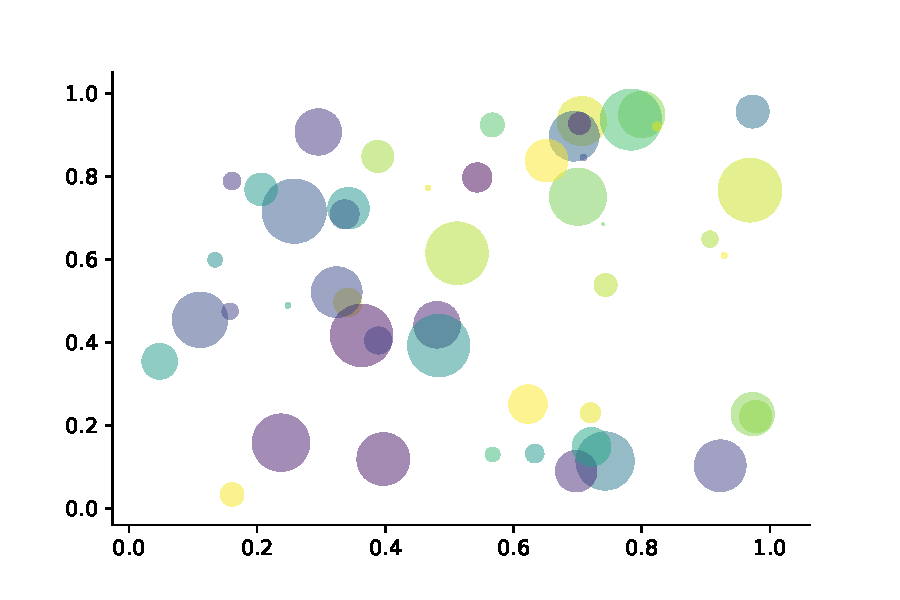
\includegraphics[width=0.6\textwidth]{figure/scatter.pdf}
	\caption{Matplotlib: Scatter Plot Example\label{fig:scatter}}
\end{figure}

\begin{table}[t]
  \small
  \centering
  \caption{Auto MPG and Price \label{tab:reg}}
    \begin{tabular}{lcc}
    \toprule
                    &       (1)         &        (2)      \\
    \midrule
    mpg             &    -238.90***     &      -49.51     \\
                    &     (53.08)       &      (86.16)    \\
    weight          &                   &      1.75***    \\
                    &                   &      (0.641)    \\
    constant        &     11,253***     &       1,946     \\
                    &     (1,171)       &      (3,597)   \\
    obs             &        74         &         74     \\
    $R^2$           &      0.220        &       0.293    \\
    \bottomrule
    \multicolumn{3}{l}{\scriptsize Standard errors in parentheses} \\
    \multicolumn{3}{l}{\scriptsize *** p<0.01, ** p<0.05, * p<0.1} \\
    \end{tabular}%
\end{table}%

\section{List Environments}

This template uses \lstinline{tikz} to customize the list environments, with \lstinline{itemize} environment customized to the third depth and \lstinline{enumerate} environment customized to fourth depth. The effect is as follows\\[2ex]
\begin{minipage}[b]{0.49\textwidth}
\begin{itemize}
   \item first item of nesti;
   \item second item of nesti;
   \begin{itemize}
      \item first item of nestii;
      \item second item of nestii;
      \begin{itemize}
         \item first item of nestiii;
         \item second item of nestiii.
      \end{itemize}   
   \end{itemize}
\end{itemize}
\end{minipage}
\begin{minipage}[b]{0.49\textwidth}
\begin{enumerate}
   \item first item of nesti;
   \item second item of nesti;
   \begin{enumerate}
      \item first item of nestii;
      \item second item of nestii;
      \begin{enumerate}
         \item first item of nestiii;
         \item second item of nestiii.
      \end{enumerate}   
   \end{enumerate}
\end{enumerate}
\end{minipage}

\subsection{Diagrams}

\begin{sequencediagram}
\newinst{ue}{UE}
\newinst[3]{nodeb}{Node B}
\newinst[3]{rnc}{RNC}
\mess{ue}{RRC Connection Request}{rnc}
\mess{rnc}{Radio Link Setup Request}{nodeb}
\mess{nodeb}{Radio Link Setup Response}{rnc}
\mess{rnc}{Establish Request}{nodeb}
\mess{nodeb}{Establish Confirm}{rnc}
\mess{rnc}{RRC Connection Setup}{ue}
\postlevel
\mess{nodeb}{Synchronization Indication}{rnc}
\filldraw[fill=black!30] ($(RRC Connection Setup to)+(0,-.3)$) rectangle ($(Synchronization Indication from) +(0,.3)$)
 node[midway] {L1 Synchronization};
\mess{ue}{RRC Connection Setup Complete}{rnc}
\end{sequencediagram}
